\chapter{Some preliminaries}

A citation to \cite{lundell2009transformation} and \cite{lundell2009some} for the sake of illustration.

\begin{definition}
    A definition can be used to define things.
\end{definition}

\begin{theorem}
    Here is a theorem with proof with an equation
        \begin{equation}
            a+b=c.
        \end{equation}
\end{theorem}

\begin{proof}
Test
\end{proof}

\begin{lemma}
    A lemma.
\end{lemma}

\begin{remark}
    A remark.
\end{remark}

\begin{example}
    Here is also an example.
\end{example}

\blindmathfalse
\Blindtext

\begin{figure}[t]
    \centering
    \includegraphics[width=4cm]{sigill.png}
    \caption{This is the official seal of {\AA}bo Akademi University.}
    \label{fig:my_figure}
\end{figure}

\Blindtext

\begin{figure}[tb]
    \centering
    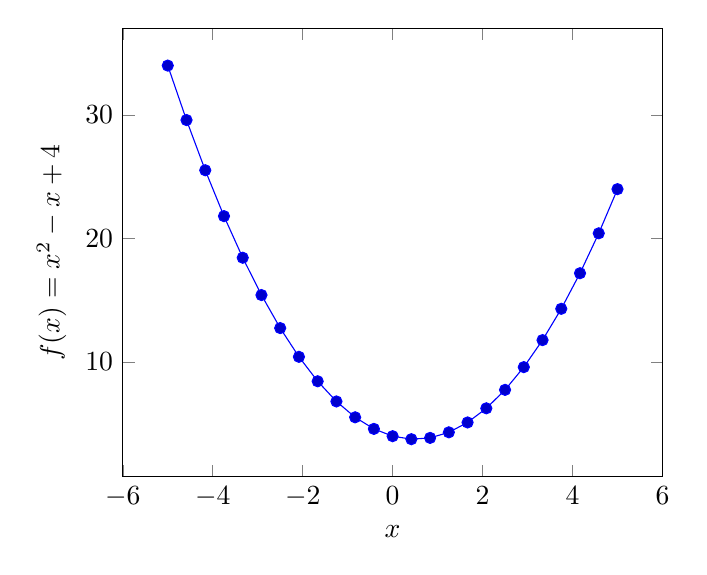
\begin{tikzpicture}
    	\begin{axis}[
    		xlabel=$x$,
    		ylabel={$f(x) = x^2 - x +4$}
    	]
    	% use TeX as calculator:
    	\addplot {x^2 - x +4};
    	\end{axis}
    \end{tikzpicture}
    \caption{Use \texttt{pgfplots} for simple and not so simple plots.}
    \label{fig:my_plot}
\end{figure}

\Blindtext


\begin{table}[t]
    \centering
    \begin{tabular}{ l c r }
      1 & 2 & 3 \\
      4 & 5 & 6 \\
      7 & 8 & 9 \\
    \end{tabular}
    \caption{This is a table.}
    \label{fig:my_table}
\end{table}

